The training loss plot for $CAD_{DL}$ is shown in Figure \ref{fig:5}. In the two folds, the CNN reduces the loss abruptly within the first few iterations and the learning process becomes gradual as the training continues. This trend is repeated in Table \ref{tab:table2}, where the increase in AUC becomes more incremental as the number of epochs increases plateauing at epoch 5. On the other hand, the detection rate at 0.1 false-postive rate (FPR) increases with increasing margin until it reaches maximums at epoch 5. All the models have a higher AUC and all except the model at epoch-1 have a higher detection rate at 0.1 FPR than $CAD_{SVM}$.

\begin{figure} [ht]
   \begin{center}
   \begin{tabular}{c}
   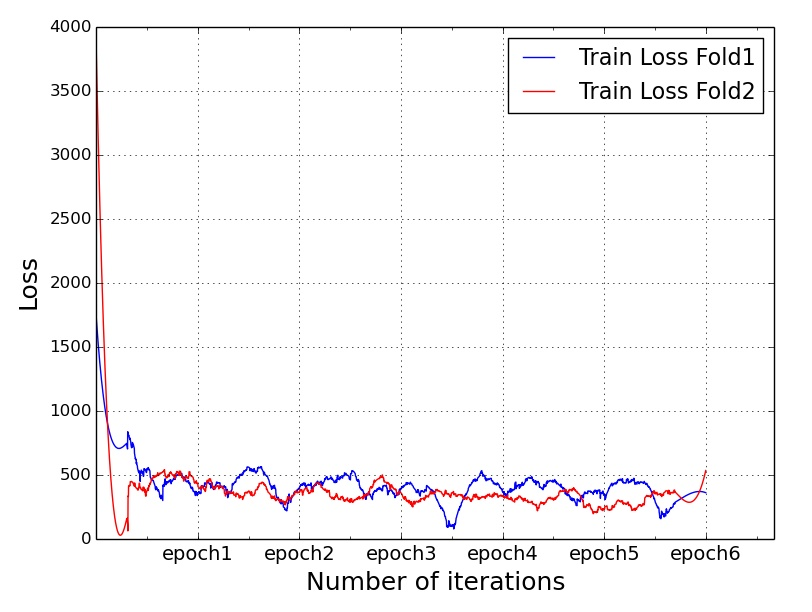
\includegraphics[height=7.5cm]{Figure5}
   \end{tabular}
   \end{center}
   \caption[Fig5]
   { \label{fig:5} 
Training loss plot for the two folds in a two fold cross-validation. A filter was used to smooth out the noisy loss values for a final output.}
   \end{figure}

\begin{table}[ht]
\centering
\caption{Detection rates at 0.1 false-positive rates (FPR) and AUCs for ROC curves of all models from $CAD_{DL}$ and the competing CAD by Ref. \citenum{kwak2015automated}} 
\label{tab:table2}
\begin{center}       
\begin{tabular}{|l|l|l|} 
\hline
\rule[-1ex]{0pt}{3.5ex} Model Name &	Detection at 0.1 FPR &	AUC \\
\hline
\rule[-1ex]{0pt}{3.5ex} $CAD_{DL}$ Epoch 1 &	0.597 &	0.876 \\
\hline
\rule[-1ex]{0pt}{3.5ex} $CAD_{DL}$ Epoch 2 &	0.620 &	0.885 \\
\hline
\rule[-1ex]{0pt}{3.5ex} $CAD_{DL}$ Epoch 3 &	0.654 &	0.891 \\ 
\hline
\rule[-1ex]{0pt}{3.5ex} $CAD_{DL}$ Epoch 4 &	0.711 &	0.894 \\ 
\hline
\rule[-1ex]{0pt}{3.5ex} $CAD_{DL}$ Epoch 5 &	\textbf{0.735} &	\textbf{0.897} \\ 
\hline
\rule[-1ex]{0pt}{3.5ex} $CAD_{DL}$ Epoch 6 &	\textbf{0.735} &	\textbf{0.897} \\ 
\hline
\rule[-1ex]{0pt}{3.5ex} Kwak et. al &	0.617 &	0.859 \\ 
\hline
\end{tabular}
\end{center}
\end{table}

The ROC plots for four different models are presented in Figure \ref{fig:6}. The first three are for $CAD_{DL}$ models at different epochs, and the last curve is for $CAD_{SVM}$. As the model continues to train, $CAD_{DL}$ curves move toward the y-axis, while simultaneously showing lower detection values for higher FPRs: at 0.3 FPR epoch-1 has the highest performance with 0.92 detection rate while epoch-6 has the highest performance at 0.1 FPR with 0.731 detection rate. Furthermore, the model at epoch-6 is either equivalent to or outperforms $CAD_{SVM}$ at every FPR while the other two $CAD_{DL}$ models have an inferior performances for low FPRs.     
\begin{figure} [ht]
   \begin{center}
   \begin{tabular}{c}
   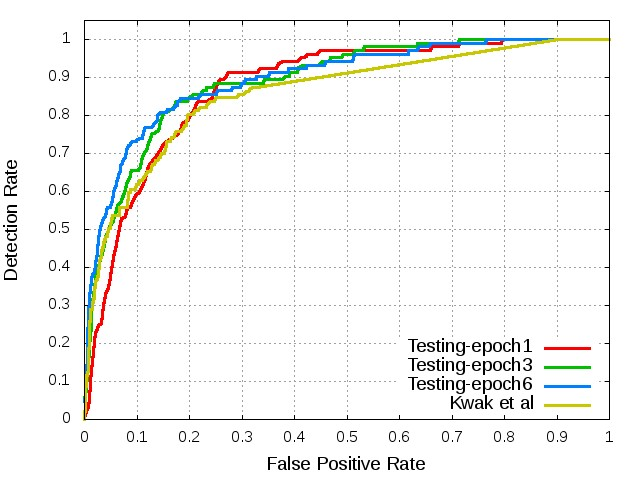
\includegraphics[height=7.5cm]{Figure6}
   \end{tabular}
   \end{center}
   \caption[Fig6]
   { \label{fig:6} 
ROC curves for  $CAD_{DL}$ at the multiple training stages denoted by epochs and for competing CAD by Kwak et. al. (Ref. \citenum{kwak2015automated}).}
   \end{figure}
A trend is apparent when inspecting the FROC curves for clinically significant lesions, which have a Gleason score of 7 or above. As shown in Figure \ref{fig:7}, with increasing epoch number the performance of $CAD_{DL}$ increases. The model at epoch-6 shows the best performance with 0.94 detection rate at a 10 false-positives per patient. This model is either equivalent to or outperforms $CAD_{SVM}$ for all FPRs while the epoch-1 model has an inferior performance with a 0.80 detection rate as compared to $CAD_{SVM}$'s  0.85 for 10 false-positives per patient. 

\begin{figure} [ht]
   \begin{center}
   \begin{tabular}{c}
   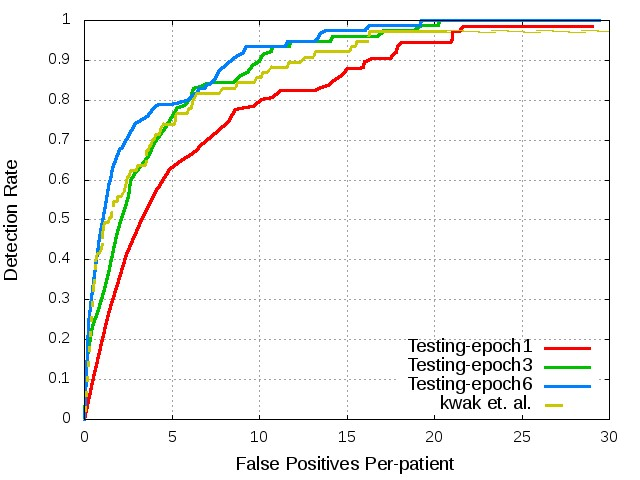
\includegraphics[height=7.5cm]{Figure7}
   \end{tabular}
   \end{center}
   \caption[Fig7]
   { \label{fig:7} 
   FROC curves for both $CAD_{DL}$ and the competing CAD by Kwak et. al (Ref. \citenum{kwak2015automated}) for clinically significant tumors (Gleason Score $\geq$ 7.)}
   \end{figure}

Figures \ref{fig:8}-\ref{fig:11} give insight into the qualitative performance of the CADs. Figure \ref{fig:8} shows a detection of a transition zone lesion that appears suspicious on all MR sequences --lesions usually have low intensity on T2W and ADC images while appearing bright on B2000. $CAD_{DL}$ detects it with high confidence while generating no false-positives. $CAD_{SVM}$ has a true-positive detection as well, but presents false-positive detections visible in the peripheral zone. 
\begin{figure} [ht]
   \begin{center}
   \begin{tabular}{c}
   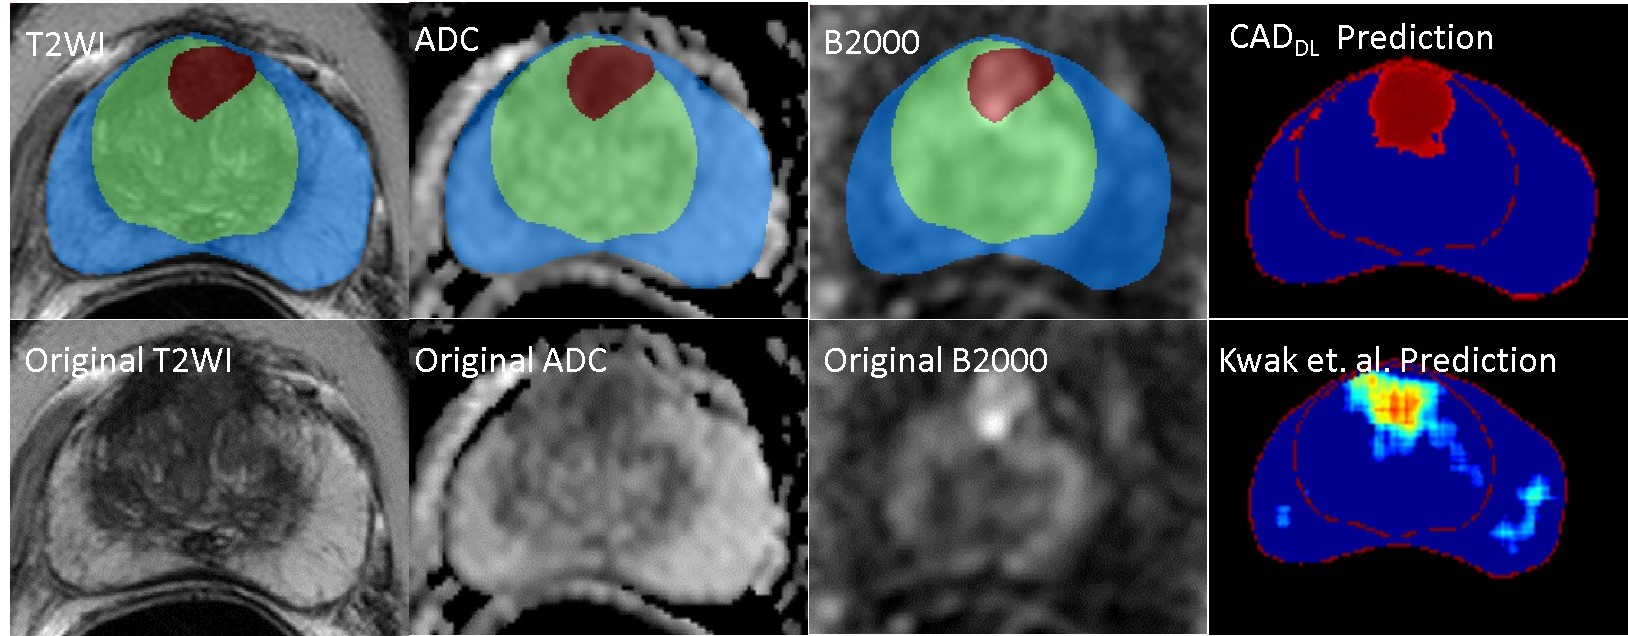
\includegraphics[height=5cm]{Figure8}
   \end{tabular}
   \end{center}
   \caption[Fig8]
   { \label{fig:8} 
An example of a true-positive detection. The top row presents the prostate mask (blue), central gland (green), and ground-truth tumor (red) overlaid upon the T2W, ADC, and B2000 images respectively. The corresponding raw T2W, ADC, and B2000 images are shown in the bottom row. Prediction heat-maps from $CAD_{DL}$ and the competing CAD by Kwak et. al (Ref. \citenum{kwak2015automated}) are placed in the last column.}
   \end{figure}
Benign prostatic hyperplasia (BPH) can be erroneously identified as cancerous by both CADs as illustrated in Figure \ref{fig:9}. However, in this instance only $CAD_{DL}$ manages to generate high probability values for the peripheral zone lesion that cohabits this region of the prostate. 
\begin{figure} [ht]
   \begin{center}
   \begin{tabular}{c}
   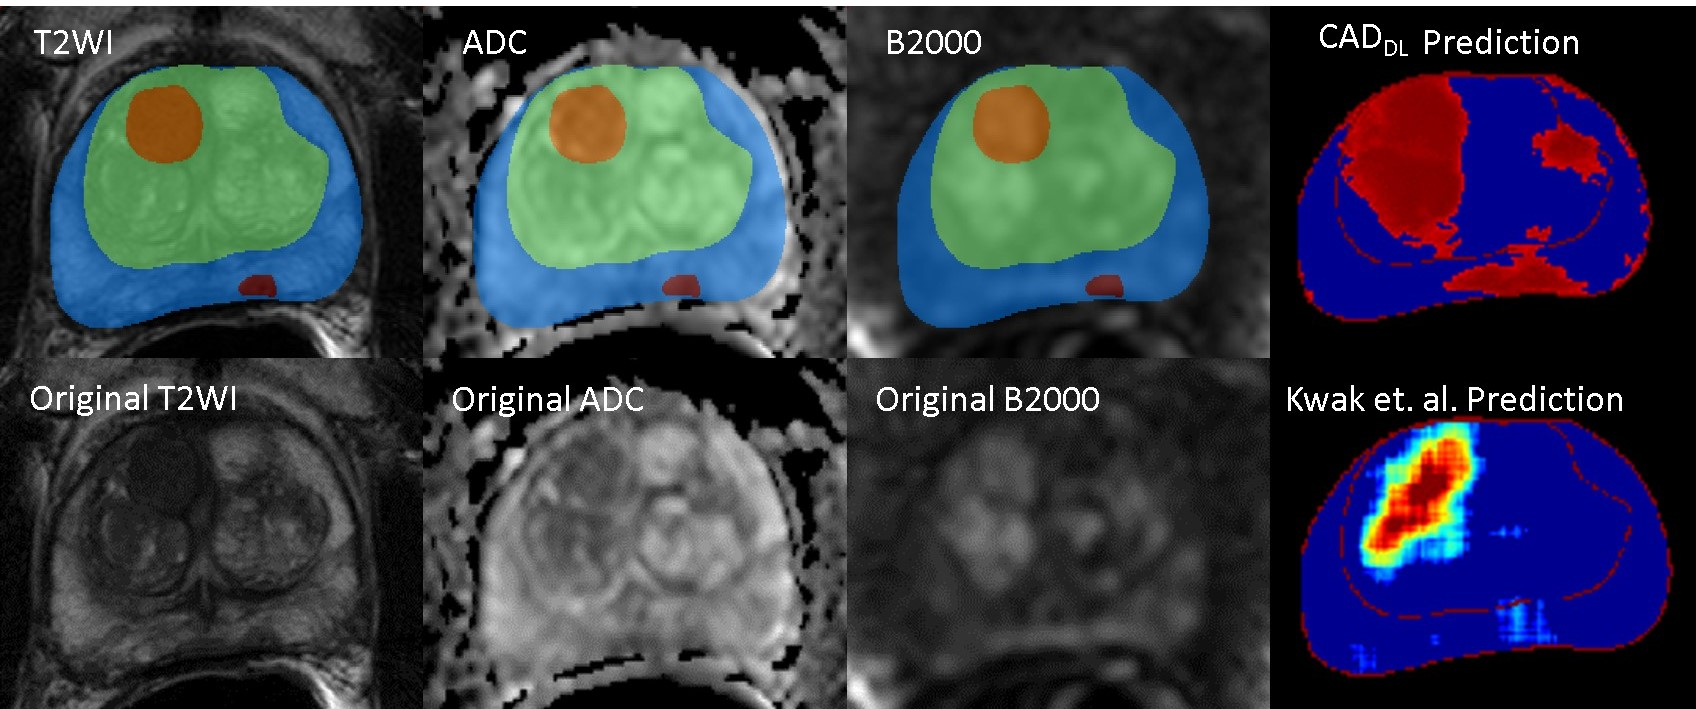
\includegraphics[height=5cm]{Figure9}
   \end{tabular}
   \end{center}
   \caption[Fig9]
   { \label{fig:9} 
An example of a benign prostatic hyperplasia (BPH) and a lesion detection. The top row displays the prostate mask (blue), central gland (green), ground-truth tumor (red), and BPH (orange) overlaid upon the T2W, ADC, and B2000 images respectively. The corresponding raw T2W, ADC, and B2000 images are shown in the bottom row. Prediction heat-maps from $CAD_{DL}$ and the competing CAD by Kwak et. al (Ref. \citenum{kwak2015automated}) are in the last column.}
   \end{figure}
Some lesions can be difficult to identify for the CADs, such as the small peripheral zone tumor presented in Figure \ref{fig:10}. In this example, both CADs incorrectly predict a large tumor in the transition zone where there are no marked regions of interest.   
\begin{figure} [ht]
   \begin{center}
   \begin{tabular}{c}
   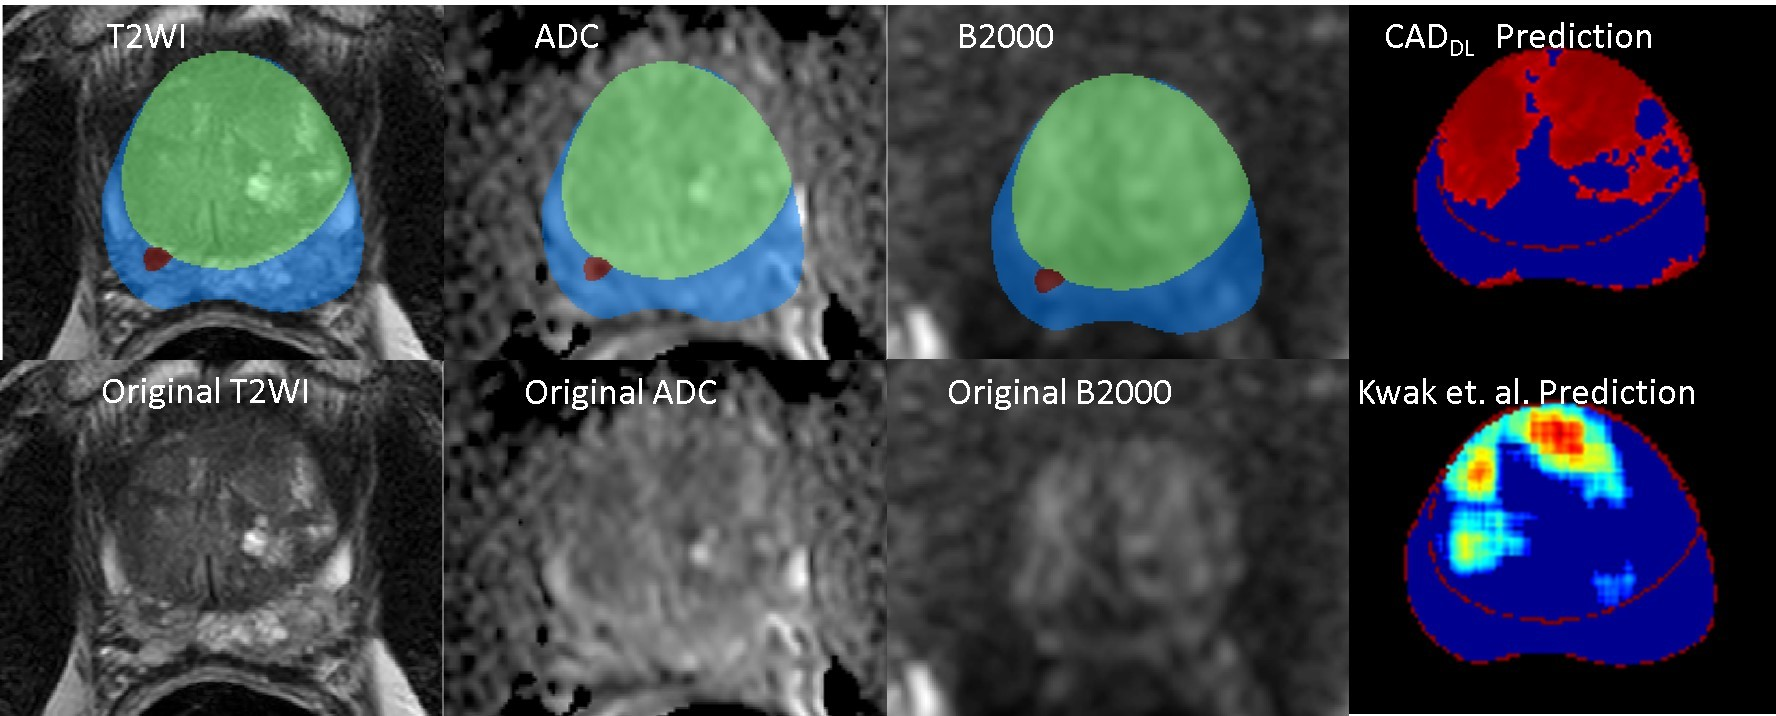
\includegraphics[height=5cm]{Figure10}
   \end{tabular}
   \end{center}
   \caption[Fig10]
   { \label{fig:10} 
An example of a true-negative and a false-positive detection. The top row has the prostate mask (blue), central gland (green), and ground-truth tumor (red) displayed over T2W, ADC, and B2000 images respectively. The corresponding raw T2W, ADC, and B2000 images are shown in the bottom row. Prediction heat-maps from $CAD_{DL}$ and the competing CAD by Kwak et. al (Ref. \citenum{kwak2015automated}) are placed in the last column.}
   \end{figure}
Lastly, false predictions can also arise from an artifact within the image. Figure \ref{fig:11} presents an example where there is a blurry region in the peripheral zone of the T2W image. $CAD_{DL}$ incorrectly predicts suspicion in this region with high probability while $CAD_{SVM}$ remains largely unaffected by the low quality image.   
\begin{figure} [ht]
   \begin{center}
   \begin{tabular}{c}
   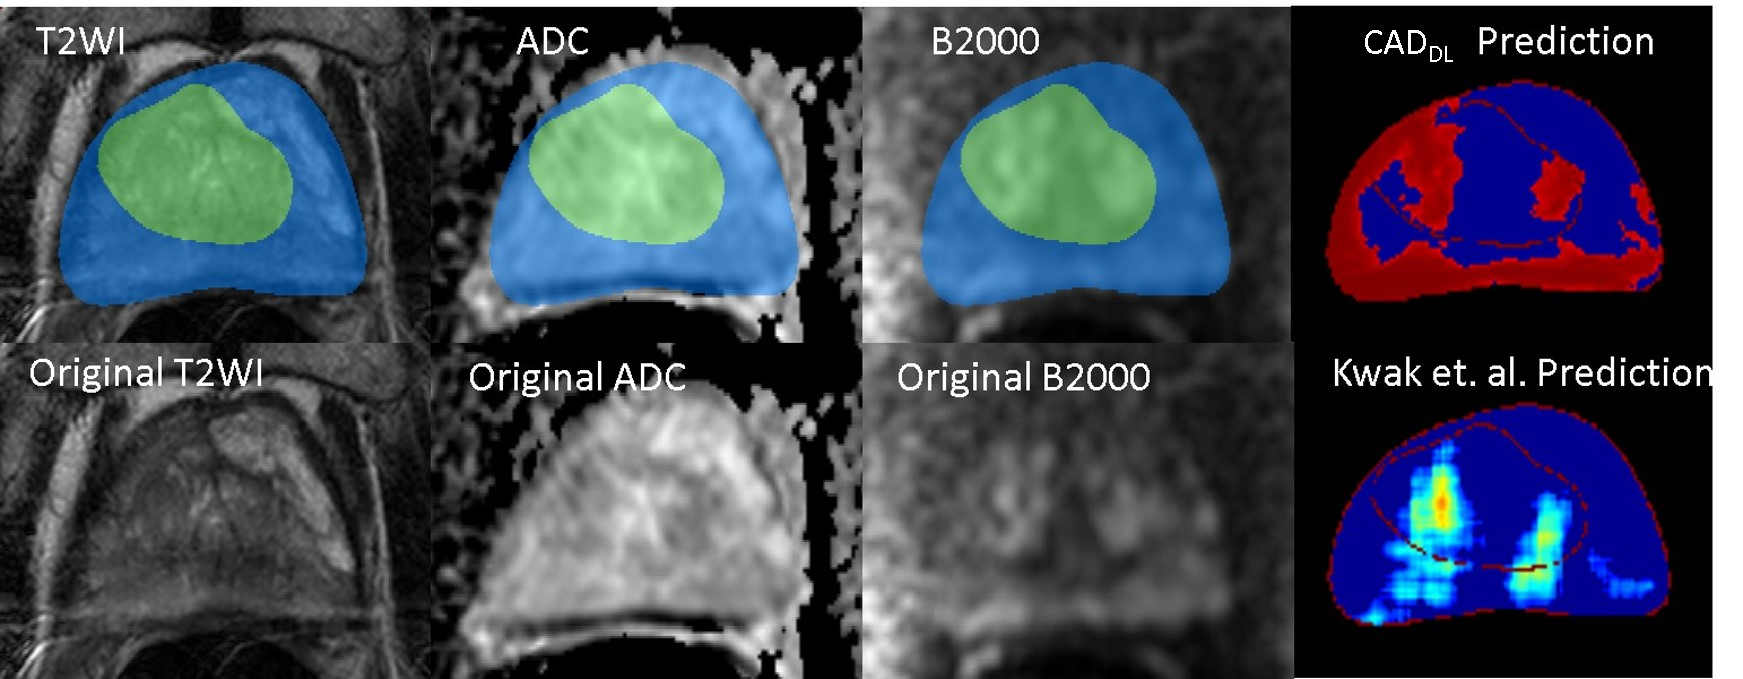
\includegraphics[height=5cm]{Figure11}
   \end{tabular}
   \end{center}
   \caption[Fig11]
   { \label{fig:11} 
An example of a false-positive detection arising from what may be an artifact within the T2W image. The top row presents the prostate mask (blue), and central gland (green) overlaid T2W, ADC, and B2000 images respectively. The corresponding raw T2W, ADC, and B2000 images are shown in the bottom row. Prediction heat-maps from $CAD_{DL}$ and the competing CAD by Kwak et. al (Ref. \citenum{kwak2015automated}) are placed in the last column.}
   \end{figure}

